\documentclass[12pt]{article}
\usepackage{listings}
\usepackage{xcolor}

\lstdefinestyle{customc}{
  belowcaptionskip=1\baselineskip,
  breaklines=true,
  frame=L,
  xleftmargin=\parindent,
  language=C,
  showstringspaces=false,
  basicstyle=\footnotesize\ttfamily,
  keywordstyle=\bfseries\color{green!40!black},
  commentstyle=\itshape\color{purple!40!black},
  identifierstyle=\color{blue},
  stringstyle=\color{orange},
}

\lstdefinestyle{customasm}{
  belowcaptionskip=1\baselineskip,
  frame=L,
  xleftmargin=\parindent,
  language=[x86masm]Assembler,
  basicstyle=\footnotesize\ttfamily,
  commentstyle=\itshape\color{purple!40!black},
}

\lstset{escapechar=@,style=customc}
\newcommand{\includecode}[1]{\lstinputlisting[frame=single]{#1}}
\newcommand{\code}[1]{\emph{#1}}

\usepackage{booktabs}
\usepackage{pgfplotstable}

\usepackage{sbc-template}
\usepackage{graphicx,url}

\usepackage[brazil]{babel}   
%\usepackage[latin1]{inputenc}  
\usepackage[utf8]{inputenc}  

%%%%%%%%%%%%%%%%%%%%%%%%%%%%%%%%%%%%%%%%%%%%%%%%%%%%%%%%%%%%%%%%%%%%%%%    
     
\sloppy

\title{O Heap é a Minha Esperança}

\author{Micael Levi Lima Cavalcante - 21554923}


\address{Instituto da Computação -- Universidade Federal do Amazonas (UFAM)\\
  Av. General Rodrigo Octávio, 6200 -- Coroado I -- Manaus -- AM -- Brasil
  \email{mllc@icomp.ufam.edu.br}
}

\begin{document} 

\maketitle

\section{Experimento}

\subsection{Tipos de ordenação}

%Explique o passo-a-passo para uso dos tipos abstrato implementado. Meça o tempo de execução do programa. Em quanto tempo, em segundos, toda a carga de trabalho foi processada? Quantas movimentações foram realizadas por operação, na média?

Na linguagem C esse processo é realizado criando um arquivo cabeçalho que contém a interface do TAD, ou seja, a implementação fica em outro arquivo (conhecido como módulo) que será \emph{linkado} com o respectivo cabeçalho. E este último estará incluso no único arquivo que irá usar diretamente o conjunto de dados que o tipo \textbf{TFila} (que foi definido no arquivo cabeçalho da fila, independente do tipo de ordenação) manipula, o arquivo \code{servico.c}.
Com o objetivo de manipular filas de prioridade, devemos adotar conceitos de ordenação completa e ordenação parcial. Os tipos abstratos de dados utilizados foram fila e heap, respectivamente.

%%%%%%%%%%% TAD: Fila
\begin{table}[h]
\centering
\caption{TAD: Fila}
\label{table:t0}
\begin{tabular}{|ll|}
\hline
\textbf{enfileirar(fila, elemento)} & insere elemento no fim da fila e ordena de acordo com a sua prioridade \\ \hline
\textbf{desenfileirar(fila)}        & retira o primeiro elemento da fila (maior prioridade)                  \\ \hline
\textbf{vazia(fila)}                & verifica se a fila está vazia                                          \\ \hline
\end{tabular}
\end{table}

Com o TAD definido, podemos implementá-lo em linguagem C salvando como \code{fila.h} (interface):

\begin{lstlisting}[frame=single]

typedef short (*TEnfileirar)(TFila*,void*);
typedef void* (*TDesenfileirar)(TFila*);
typedef short (*TVazia)(TFila*);
typedef void (*TAnalytics)(TFila*);

TFila *criarFila();
void destruirFila(TFila*);

struct fila{
    void *dado;

    TEnfileirar enfileirar;
    TDesenfileirar desenfileirar;
    TVazia vazia;
    TAnalytics analytics;
};
\end{lstlisting}


Visualizando somente essa interface, não é possível identificar como as operações são realizadas. Para usar a fila de prioridade, temos que implementar o \code{fila.c} de acordo com seguintes regras para cada tipo de ordenação.

\begin{figure}[h!]
\centering
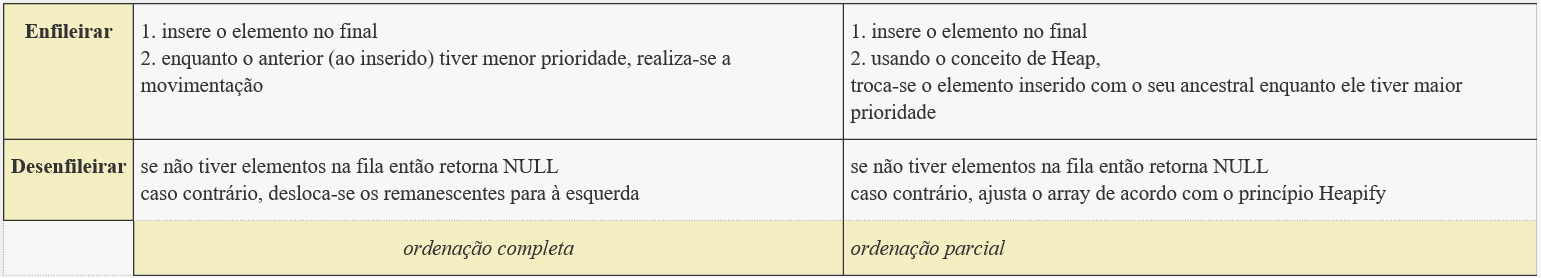
\includegraphics[width=1.1\textwidth]{algoritmo.png}
\caption{Relação de utilização dos arquivos}
\label{fig:relacoes}
\end{figure}


%%%%%%%% TABELA (TAD) tempo x instancia
\begin{figure}[h!]
\centering
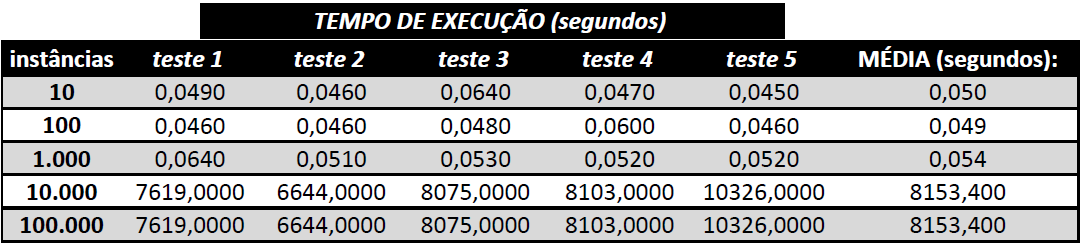
\includegraphics[width=1.1\textwidth]{tabela_parcial.PNG}
\caption{TAD Fila - tabela relação instância x tempo}
\label{fig:t1}
\end{figure}

%A figura a seguir mostra o tempo de execução do mesmo programa mas utilizando a ordenação parcial com Heap.
%%%%%%%% TABELA (TAD) tempo x instancia
%\begin{figure}[h!]
%\centering
%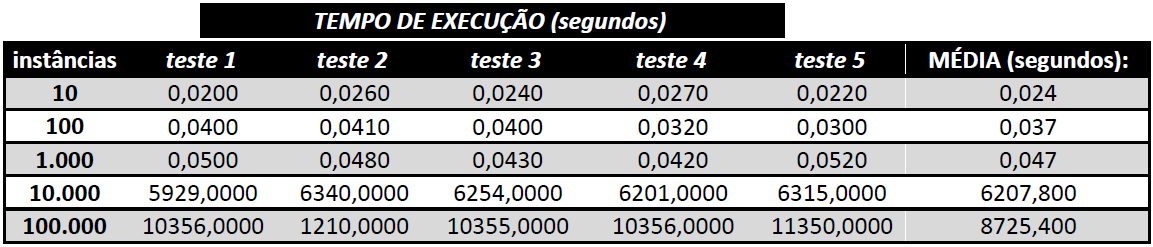
\includegraphics[width=1.1\textwidth]{tabela_completa.png}
%\caption{TAD Heap - tabela relação instância x tempo}
%\label{fig:t1}
%\end{figure}


%%%%%%%% TABELA (TAD) movimentações x instancia
\begin{figure}[h!]
\centering
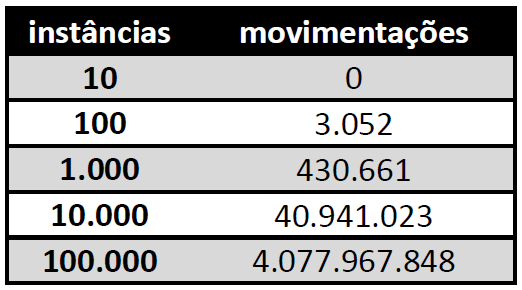
\includegraphics[width=.4\textwidth]{movimentacoes_parcial.PNG}
\caption{TAD Fila - tabela da relação movimentação x instância}
\label{fig:t2}
\end{figure}


\subsection{A configuração experimental}
%Mostre como o experimento foi realizado. Use figuras esquemáticas para mostrar os componentes da sua implementação, destacando como eles se conectam. Explique como os TADs devem ser utilizados.

Para iniciar o uso de qualquer um dos TADs expostos acima, deve-se seguir os passos abaixo.

\begin{enumerate}
    \item Dado um código-fonte, devemos incluir a interface da fila, por exemplo:
\begin{lstlisting}[frame=single]
#include "fila.h"
\end{lstlisting}

Assim temos acesso a um conjunto de operações básicas que atuarão somente nos dados referente à fila, independente do tipo de elemento que será inserido.

    \item Para criarmos uma instância da fila, chamamos a função que retorna um ponteiro para o tipo \textbf{TFila}, como por exemplo:
\begin{lstlisting}[frame=single]
TFila* minha_fila = criarFila();
\end{lstlisting}

    \item Então podemos inserir e remover, respectivamente, um elemento nessa fila, basta acessar o método que possui tais funções, e.g.:
\begin{lstlisting}[frame=single]
int meuDado = 4;
minhaFila->enfileirar(minhaFila, &meuDado);
int *removido = minhaFila->desenfileirar(minhaFila);
\end{lstlisting}
\end{enumerate}

\begin{figure}[h!tb]
\centering
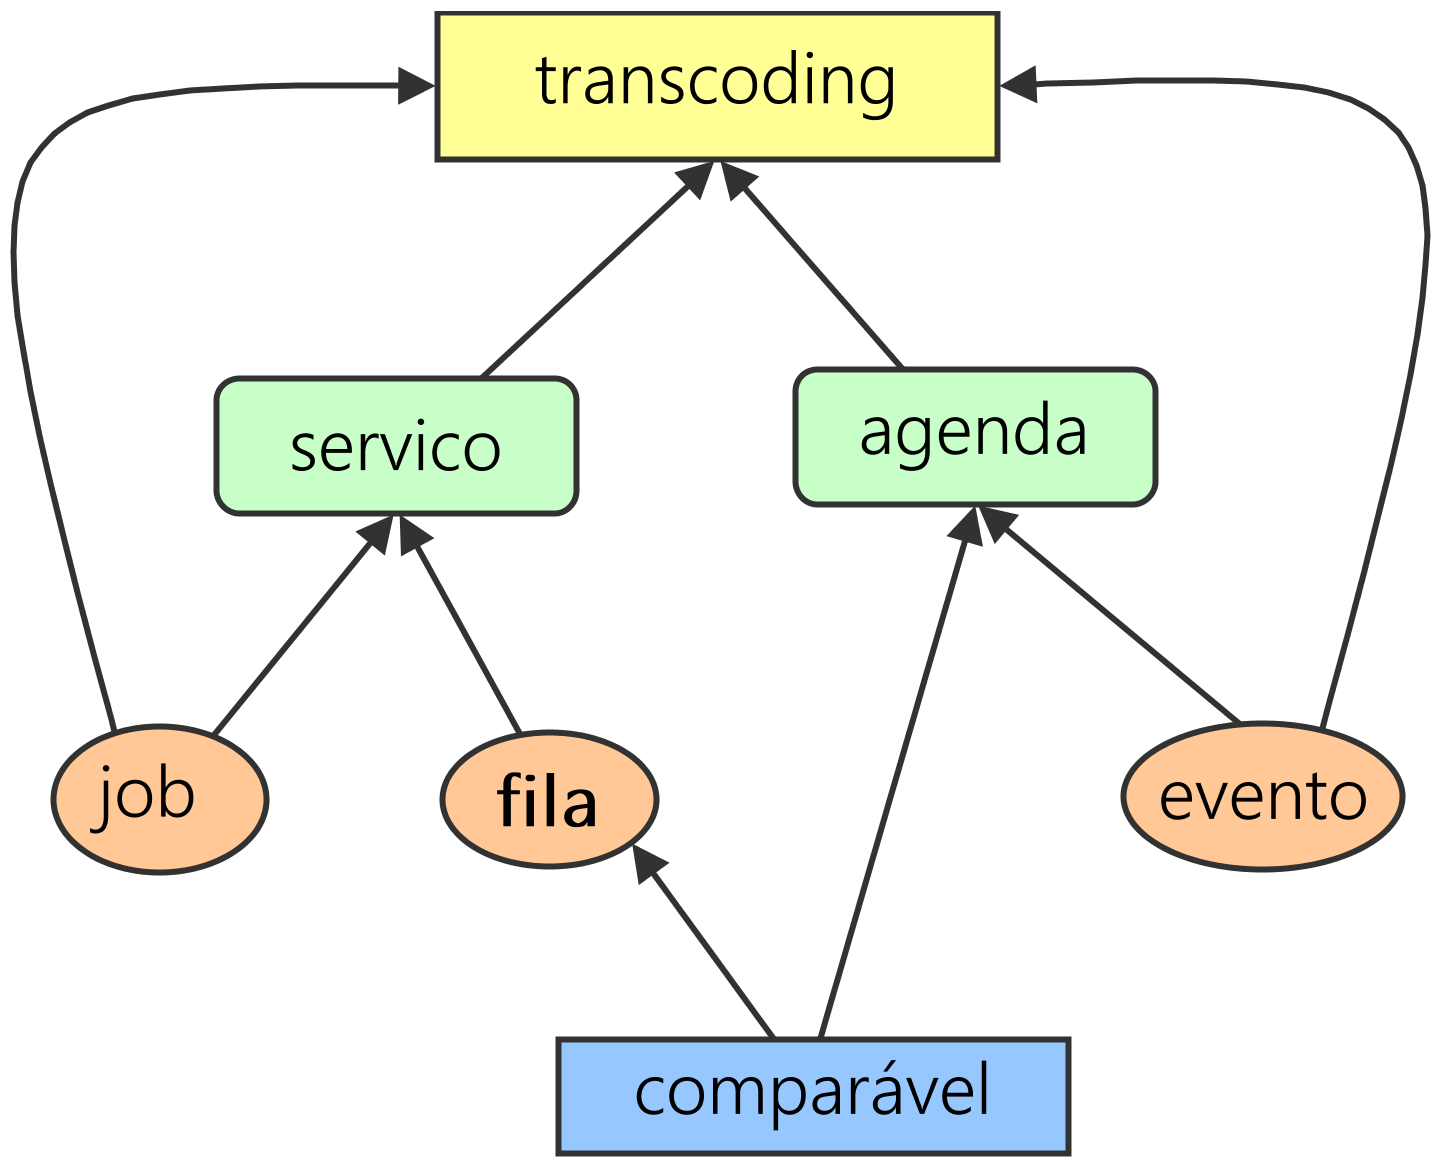
\includegraphics[width=.5\textwidth]{relacao_cabecalhos.png}
\caption{Relação de utilização dos arquivos}
\label{fig:cabecalhos}
\end{figure}
A figura (\ref{fig:cabecalhos}) acima abstrai as relações de conexão entre o tipo abstrato que é implementado no arquivo \emph{fila.c} com os outros módulos do programa. Podemos ver que a fila é acessível "diretamente" apenas pelo conjunto de operações contidos no módulo \email{servico.c}, porém, ainda sim, o modelo de dados implementado, o conteúdo da fila e todo o processo de manipulação da mesma não são expostos. Para usá-la é preciso. Assim, temos o aumento da eficiência do programa e redução de erros pois a única conexão entre o TAD utilizado e o restante do programa é aquela constituída pela interface imutável dos algoritmos que implementam a estrutura ativa do TAD. Os outros módulos podem utilizar essa interface através do único laço de conexão que foi estabelecido entre o \emph{servico} e o \emph{fila}.

A implementação efetiva pode ser feita buscando a cumprir os objetivos das operações vistas na tabela \ref{table:t0} da página \pageref{table:t0}. Praticamente a única diferença da implementação entre os dois tipos está na forma de ordenação, ou seja, ao inserir e retirar um elemento da fila, precisamos ordenar de acordo com o TAD em uso (como foi definido na figura \ref{fig:cabecalhos}.

\begin{enumerate}
    \item Definindo o tipo de dado que será armazenado na estrutura de dados vetor, na ordenação parcial:
\begin{lstlisting}[frame=single]
typedef struct{
	void** fila;
	unsigned tamanho;

	int primeiro;
	int ultimo;
	TStatsFila stats;
} TDadoFila;
\end{lstlisting}

    \item Na ordenação completa ficaria:
\begin{lstlisting}[frame=single]
typedef struct{
	void** fila;
	unsigned tamanho;

  int ocupacao;

	TStatsFila stats;
} TDadoFila;
\end{lstlisting}
\end{enumerate}

Para a ordenação parcial, a parte quee lida com as inserções e remoções ficou da forma:
\begin{lstlisting}[frame=single]
static void* Desenfileirar(TFila *f){
	void* elemento=NULL;
	TDadoFila *d = f->dado;

	if (d->primeiro == -1){
		elemento = NULL;
	}else{
		elemento  = d->fila[d->primeiro];
		if (d->primeiro == d->ultimo){
			d->primeiro = d->ultimo = -1;
		}else{
			int i;
			for(i=d->primeiro; i < d->ultimo; i++){
				d->fila[i] = d->fila[i+1];
			}
			d->ultimo--;
		}
		d->stats.removeu++;
		d->stats.movimentou
		+= (d->ultimo-d->primeiro)+(d->primeiro==-1?0:1);
	}
	return elemento;
}


static short Enfileirar(TFila *f, void *elemento){
	TDadoFila *d = f->dado;
	int posInsercao = d->ultimo+1, i;
	void *aux;

	if(d->primeiro == -1){
		d->primeiro = d->ultimo = 0;
		d->fila[d->primeiro] = elemento;
	}else{
		if(posInsercao >= d->tamanho) ajustarFila(f, posInsercao*2);

		d->ultimo = posInsercao;
		d->fila[posInsercao] = elemento;

		for(i=posInsercao; (i > 0) &&
		COMPARAR_PRIORIDADES(d->fila[i-1], d->fila[i]); i--){
			aux 		=	d->fila[i];
			d->fila[i] 	= d->fila[i-1];
			d->fila[i-1]= aux;
			d->stats.movimentou++;
		}
	}
	d->stats.inseriu++;
	return 1;
}
\end{lstlisting}


Para a ordenação completa, mudamos para:
\begin{lstlisting}[frame=single]
static void* Desenfileirar(TFila *f){
	if(Vazia(f)) return NULL;
	TDadoFila *d = f->dado;

  void *raiz = d->fila[0], **vet = d->fila;
  int posUltimo = d->ocupacao - 1;

  if(posUltimo > 0){
    vet[0]         = vet[posUltimo];
    vet[posUltimo] = raiz;

    d->stats.movimentou++;

    d->ocupacao--;
    posUltimo = d->ocupacao-1;

    if(posUltimo > 0) ajustarHeap(d, vet, 0, posUltimo);
  }
	d->stats.removeu++;
	return raiz;
}


static short Enfileirar(TFila *f, void *elemento){
	TDadoFila *d = f->dado;
    int i=d->ocupacao, posAncestral;
	void *aux;

	if(i >= d->tamanho) ajustarFila(f, i*2);

  d->fila[i] = elemento;
  d->ocupacao=i+1;

  posAncestral = PAI(i);

  while( (i > 0)
  && (COMPARAR_PRIORIDADES(d->fila[posAncestral],d->fila[i])) ){
    aux 				=	d->fila[posAncestral];
    d->fila[posAncestral] = d->fila[i];
    d->fila[i]            = aux;

    d->stats.movimentou++;

    i = posAncestral;
	posAncestral = PAI(i);
  }

	d->stats.inseriu++;
	return 1;
}
\end{lstlisting}





\section{Resultados e interpretações} \label{sec:firstpage}

%Mostre o gráfico com o resultado coletados para movimentação de elementos com as diferentes instancias do problema. Isto é, um gráfico de linha que mostre a relação entre o tamanho da instancia e o numero de movimentações. As cargas de trabalho serão montadas para explorar diferentes aspectos de implementação da fila e do heap. É preciso considerar que as movimentações são geradas por inclusões e remoções, portanto é importante que o efeito dessas operações esteja claramente identificados. Apresente um relação teoria com a prática. Quão exato foi a análise assintótica para o problema em questão?

A ordenação total é realiza utilizando o algoritmo de Ordenação por Inserção. Essa ordenação só é realizada quando enfileiramos um dado na fila. É simples, estável e de fácil implementação porém possui complexidade $O(n^2)$ no pior caso, isso implica em uma execução demorada caso a fila possua muitos elementos, ou seja, se o tempo de processamento de muitos vídeos for relativamente alto. Em contrapartida, em instâncias pequenas ou com tempo de processamento muito baixo, esse tipo de ordenação pode ser eficiente, facilitando assim o processo de retiradas dos vídeos. A ordenação parcial possui uma complexidade $O(\log{}n)$ no pior caso, isso mostra que esse tipo de ordenação tende a ser melhor que a ordenação completa (para o problema em questão).

O gráfico a seguir mostra a relação das movimentações realizadas em cada instância criada a partir da figura (\ref{fig:t2}). Nele observamos a enorme diferença de movimentações entre a última e a penúltima instâncias. Isso acarreta numa diferença relativamente alta no tempo de execução do programa para essa configuração de fila.

%%%%%%%% GRÁFICO (TAD) movimentações x instancia
\begin{figure}[h!]
\centering
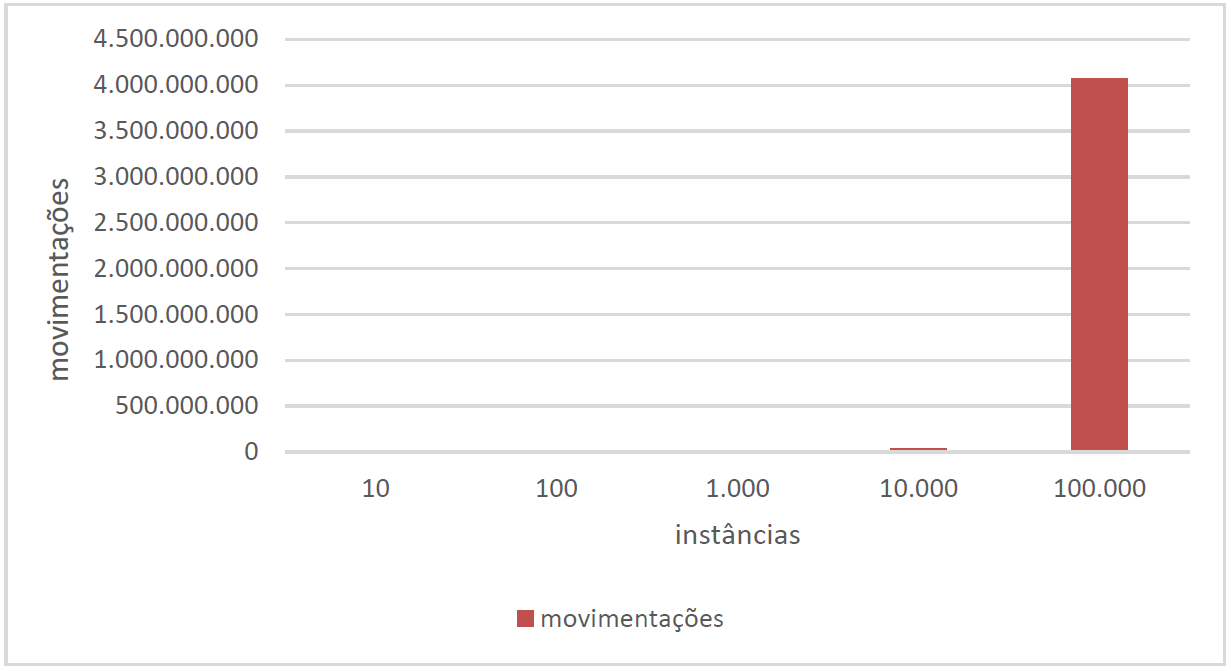
\includegraphics[width=1\textwidth]{grafico2.PNG}
\caption{TAD Fila - gráfico da relação movimentações x instância}
\label{fig:g1}
\end{figure}

\newpage


\section{Conclusão (Discussão dos resultados)}

%Discuta os resultados. Compara os valores gerados por cada operação em cada tipo de estrutura. Compare o seu resultado com o que diz a teoria. Em que cenário uma estrutura é mais adequada que outra? Em não dispondo de tempo para realizar em avaliação, qual estrutura você indicaria na sua empresa? Porquê?
Como já era esperado para essa situação-problema, a ordenação parcial é muito mais eficiente que a completa. Logo, a minha recomendação seria utilizar a estrutura do Heap pois apesar dá ideia de manter uma coleção de elementos ordenados de acordo com um valor de prioridade associado, nesse problema não precisamos ordenar todos o conjunto, visto que na maioria das instâncias testadas o tempo de transcodificação de um vídeo é muito elevada e isso implica no enfileiramento de muitos dados que depois serão removidos, e a cada remoção precisaremos deslocar $N-1$ elementos, i.e., realizar $N-1$ movimentações (onde $N$ é o tamanho da instância).


%\bibliographystyle{sbc}
%\bibliography{sbc-template}
